\documentclass[compress]{beamer}

% \mode<presentation>{
\usetheme{Singapore}
\usecolortheme{rose}
% }
% \usepackage[utf8]{inputenc}
% \usepackage{default}
% \usepackage[portuguese]{babel}
% \usepackage{pgfplots}
% \pgfplotsset{/pgf/number format/use comma,compat=newest}
% \usepackage{color}
\usepackage{amsmath,amsfonts,amssymb}
% \usepackage{hyperref}
% \usepackage{tikz}

% \usebackgroundtemplate{%
% \tikz\node[opacity=0.5] {\includegraphics[height=\paperheight,width=\paperwidth]{logoh_2.png}};}


\title{Neural Word Embedding as Implicit Matrix Factorization}
\author{Shih-Ming Wang}
\institute{NLPLab, Institute of Information Science, Academia Sinica}
\date{\today}
\subject{Computer Science}
\begin{document}
\beamertemplatenavigationsymbolsempty

\begin{frame}
 \maketitle
\end{frame}

\begin{frame}
 \frametitle{Outline}
 \tableofcontents
\end{frame}
\section{Introduction}
%%
\begin{frame}{\secname}
\begin{itemize}
  \item Word representation - why and how
  \item Distributional hypothesis
    \begin{itemize}
      \item Words in similar contexts have similar meanings
      \item Word-context matrix
    \end{itemize}
\item Skip-gram model
   	\begin{itemize}
      \item Neural-network based
      \item Represent both word and context as vector
      \item Maximize the dot-product of frequently occurring word-context vector pairs
      \item Not well (theoretically) understood
    \end{itemize}
\item Analyze skip-gram as an implicit word-context matrix factorization
\end{itemize}
\end{frame} 
\section[Skip-Gram with NS]{Skip-Gram with Negative Sampling (SGNS)}
\subsection{Skip-Gram Model}
%%
\begin{frame}{\subsecname}
	\begin{columns}[T] % contents are top vertically aligned
    	\begin{column}[T]{.6\textwidth} % each column can also be its own environment
          \begin{itemize}
            \item Words as dense vector (projected from one-hot)
            \item Different projection matrix for input and output words (context)
            \item Loss function: $\frac{1}{T}\sum\limits_{t=1}^T\sum\limits_{-c \leq j \leq c} logp(w_{t+j}|w_t) $, where $p(w_o|w_t)=\frac{exp(\vec{w}_o\cdot \vec{w}_t)}{\sum_{i=1}^{||V||}exp(\vec{w}_i\cdot \vec{w}_t)}$
            \item Problem: softmax impractical because $||V||$ is usually large 
          \end{itemize}
    	 \end{column}
     	\begin{column}[T]{.4\textwidth} % alternative top-align that's better for graphics
      		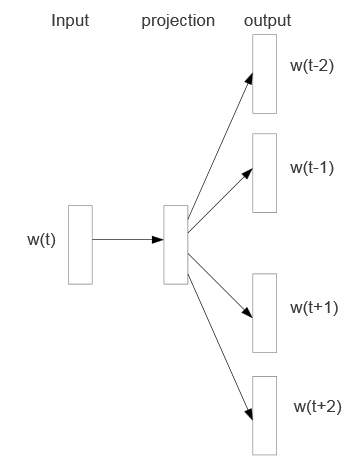
\includegraphics[height=6cm]{skip_gram.png}
     	\end{column}
     \end{columns}
\end{frame}
\subsection{Negative Sampling}
%%
\begin{frame}{\subsecname} 
  \begin{itemize}
    \item From now on, represent input and context word as $w$ and $c$
    \item Skip-Gram optimizes conditional probability $P(c|w)$
    \item Negative Sampling optimizes joint probability $P(w,c)$
    \begin{itemize}
      \item Maximize observed pairs $\sigma(\vec{w} \cdot \vec{c}) $
      \item Minimize $k$ randomly sampled negative pairs $\sigma(\vec{w} \cdot \vec{c}_N)$
      \item $\sigma(x) = \frac{1}{1+exp(-x)}$, Property: $\sigma(-x)=-\sigma(x)$
    \end{itemize}
	\item Paired-wise loss function $L(w,c)=log(\sigma(\vec{w}\cdot \vec{c})+k\mathbb{E}_{{C_N}\sim P(D)}\left [ log(\sigma(-\vec{w}\cdot \vec{c}_N)) \right ]$
    \item Global loss function: $\sum\limits_{w\in V_w}\sum\limits_{c \in V_c}\#(w,c)L(w,c)$
  \end{itemize}
\end{frame}
%%
\section[SGNS Factorization]{SGNS as Implicit Matrix Factorization}
\begin{frame}[allowframebreaks]{\secname}
	\begin{itemize}
      \item SGNS learn a (input) word embedding $W$ and a (output) context embedding $C$
      \item Rows of $W$ are used as word vectors while $C$ is usually ignored
      \item But effectively,  SGNS is implicitly factorizing a word-context matrix $M=W\cdot C^T$
      \item Each cell of $M$ equals $\vec{w}\cdot \vec{c}$, measuring the strength of association for a $(w,c)$ pair
      \item But what is the explicit form  $f(w,c)=\vec{w}\cdot \vec{c}$? 
    \end{itemize}
    \framebreak
    \begin{itemize}
      \item Assume that SGNS can fully reconstruct $M$ (this requires infinite dimension for $W$, $C$)
      \item The global loss  then equals the summation of $M$'s cells \\ $\sum\limits_{w\in V_w}\sum\limits_{c \in V_c}\#(w,c)\cdot L(w,c)$ $=\sum_i\sum_j M_{ij}=\sum_i\sum_j f(w_i,c_j)$
      \item The global loss is optimized when each cell of $M$ is optimized
      \item Goal: find explicit form $f(w,c)=\vec{w}\cdot \vec{c}$
      \item Strategy: Find $\sum\limits_{w \in V_w}\sum\limits_{c \in V_c}\ell(w,c)=\sum\limits_{w\in V_w}\sum\limits_{c \in V_c}\#(w,c)\cdot L(w,c)$, and let $\frac{\partial \ell(w,c)}{\partial (\vec{w}\cdot \vec{c})}=0$ to find $\vec{w}\cdot \vec{c}$ that optimizes $\ell(w,c)$
	\end{itemize}
     \framebreak
    \begin{itemize}
      \item  $\ell(w,c)=\#(w,c)log\sigma(\vec{w},\vec{c})+k\cdot\#(w)\cdot\frac{\#(c)}{|D|}log\sigma(-\vec{w}\cdot \vec{c})$
      \item $\vec{w}\cdot \vec{c}=log\left( \frac{\#(w,c)\cdot |D|}{\#(w)\cdot\#(c)}\right) - log~k$~(Wait, PMI?)
      \item $M^{SGNS}_{ij}=W_i\cdot C_j=\vec{w_i}\cdot \vec{c_j}=PMI(w_i, c_j)-log~k=M_{ij}^{PMI}-log~k$
      \item  $M^{SGNS}$ was assumed to be fully reconstructed (not possible)
      \item In $\ell(w,c)$, the deviation of $\vec{w_i}\cdot\vec{c_j}$ from $M^{PMI}-log~k$ is weighted by $\#(w,c)$ and $k\cdot\#(w)\cdot\frac{\#(c)}{|D|}$
      \item SGNS is a weighted matrix factorization of $M^{PMI}-log~k$
      \item Deviation of frequent word-context pairs pay more
	\end{itemize}
\end{frame}
%%
\section[Alternative]{Alternative Word Representations}
\subsection{Point-wise Mutual Information}
\begin{frame}{\subsecname}
	\begin{itemize}    
    	\item $PMI(x, y)=log\frac{P(x,y)}{P(x)P(y)}$
        \item Empirically,  $PMI(w,c)=log\frac{\#(w,c)\cdot |D|}{\#(w)\cdot \#(c)}$
        \item Issue: $M^{PMI}$ is dense 
        	\begin{itemize}
              \item For unobserved $(w,c)$, $PMI(w,c)=log0=-\infty$
              \item Solution:  $PPMI(w,c)=max(PMI(w,c), 0)$
              \item $PPMI$ lose information of infrequent word-context pairs
              \item Intuition: prefer positive ('Canada','Snow') association against negative  ('Canada','Desert') association
            \end{itemize}
       \item $M^{SGNS}=M^{PMI}-log~k$  is dense
       \item Modify: $M^{SPPMI}$ , where $SPPMI(w,c)=max(PMI(w,c)-log~k,0)$
    \end{itemize}
\end{frame}
\subsection{Singular Value Decomposition}
\begin{frame}{\subsecname}
    \begin{itemize}
        \item $M^{SPPMI}$ could directly be used as word embedding
        \item  But it's sparse, dense vectors sometimes could be better?
        \item $M^{SPPMI}=U\cdot \Sigma \cdot V^T \Rightarrow U_d\cdot \Sigma_d \cdot V^T_d = M^{SVD}$ 
        \item Choose $W^{SVD}=U_d\cdot \Sigma_d$ and $C^{SVD}=  V_d$
        \begin{itemize}
        \item Under-perform SGNS empirically
        \item $C^{SVD}$ is orthogonal while $W^{SVD}$ is not
        \item Both $C^{SGNS}$ and $W^{SGNS}$are not orthogonal
        \item $W^{SVD_{1/2}}=U_d\cdot \sqrt{\Sigma_d}$ and $C^{SVD_{1/2}}=  V_d\cdot\sqrt{\Sigma_d}$
        \item Generally $W^{SVD_{\alpha}}=U_d\cdot \Sigma^{\alpha}$(set to $1/2$ in experiments)
        \end{itemize}
    \end{itemize}
\end{frame}
%%
\section{Empirical Results}
\subsection{Experiment Setting}
\begin{frame}{\subsecname}
	\begin{itemize}
      \item Corpus: English Wikipedia, 77.5 million sentences, 1.5 billion tokens
      \item Window size is set to $5$, dropping words appears less than 100 times
      \item $189533$ terms derived for both words and contexts
    \end{itemize}
\end{frame}
\subsection{Deviation from Optimal}
\begin{frame}{\subsecname}
	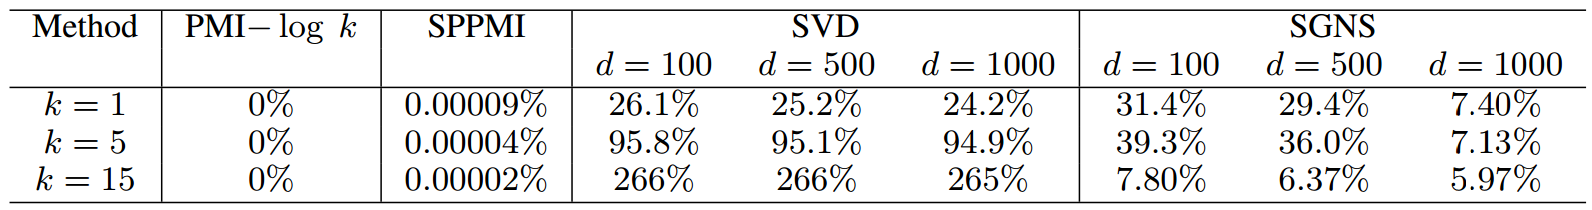
\includegraphics[height=2cm,width=\textwidth]{deviation.png}
	\begin{itemize}
    	\item The optimal solution is $PMI-log~k$
		\item SPPMI is near-perfect approximation of the optimum
		\item SVD is better when $d<500$ and $k=1$
        \item SVD fails to leverage higher dimension as SGNS does
        \item $k$'s meaning for SGNS
        \begin{itemize}
	        \item higher $k$ means more sample and better estimation of negative sample distribution (good news)
            \item higher k means that negative examples are more probable (actually not a good thing)
        \end{itemize}
		\item $SPPMI(w,c)=max(PMI(w,c)-log~k,0)$, only losing information as $k$ increases
	\end{itemize}
\end{frame}
\subsection{Linguistic Tasks}
\begin{frame}{\subsecname}
    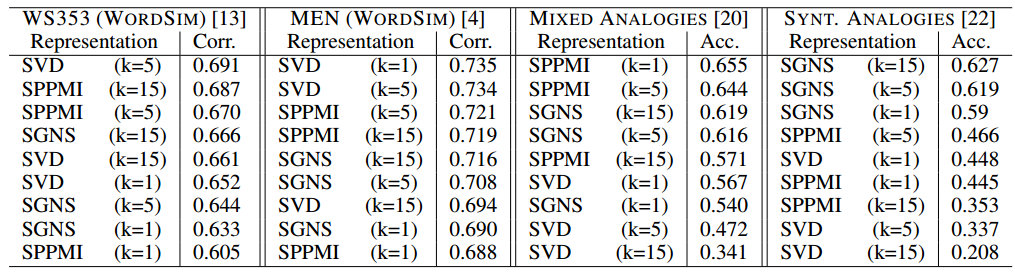
\includegraphics[height=3cm,width=\textwidth]{exp.png}
    \begin{itemize}
        \item Similarity test (WD353, Men)
        \begin{itemize}
            \item SVD $\ge$ SPPMI $\ge$ SGNS (but the difference is small)
            \item $k$ matters, SVD, SPPMI prefer small $k$, SGNS prefers large $k$
        \end{itemize}
        \item Analogies test (Mixed, Synt)
        \begin{itemize}
            \item SVD is not good
            \item SGNS significantly outperforms others on syntactic dataset
            \item Might be due to that SGNS's higher weight for frequent word such as ``the'',``will'',``each'',``had''
        \end{itemize}
    \end{itemize}
\end{frame}

\section{Conclusion}
\begin{frame}{\secname}
\begin{itemize}
    \item SGNS is shown to implicitly factorizing the $M^{PMI}-log~k$ matrix
    \item $M^{SPPMI}$, where$SPPMI=max(PMI-log~k,0)$
    \begin{itemize}
        \item Practical modification of SPMI
        \item Approximate $M^{PMI}-log~k$ better than SGNS
        \item Not necessarily performs better on linguistic tasks
        \item Might be due to SGNS's ability to perform weighted matrix factorization
    \end{itemize}
    \item SVD 
    \begin{itemize}
        \item Leads to no significantly improvement but sometimes worse performance
        \item The data is ``big'' enough to support $M^{SPPMI}$?
    \end{itemize}
    
\end{itemize}
\end{frame}

\end{document}
